\documentclass{article}
\usepackage[none]{hyphenat}
\usepackage{enumitem}
\usepackage{graphics}
\usepackage{graphicx}
\usepackage{ragged2e}
\usepackage{multirow}
\usepackage{blindtext}
\usepackage{amsmath}
\usepackage{subcaption}
\usepackage{circuitikz}
\usepackage{listings}
\usetikzlibrary{shapes.geometric}
\lstset{
	language=C++,
	basicstyle=\ttfamily\footnotesize,
	breaklines=true,
	frame=lines
	}
\title{Implementation of the below circuit using Vaman Arm}
\date{April 2023}
\author{Sai Harshith Kalithkar\\harshith.work@gmail.com\\FWC22118\\IIT Hyderabad-Future Wireless Communication Assignment-4.1}

\begin{document}
\maketitle
	\tableofcontents

\pagebreak

\section{Problem}
	{GATE EC-2019}\\
	Q.25. In the circuit shown,the clock frequency, i.e.,the frequency of the clock signal ,is 12 KHz.The frequency of the signal at Q2 is ............ KHz.
	\begin{figure}[h]
	\centering
		\begin{tikzpicture}
	\draw (0,-10) rectangle (3,-14);
	\draw (5,-10) rectangle (8,-14);
	\draw (-2,-15) -- (4,-15);
	\draw (-1,-15) -- (-1,-13.5);
	\draw (-1,-13.5) -- (0,-13.5);
	\draw (4,-15) -- (4,-13.5);
	\draw (4,-13.5) -- (5,-13.5);
	\draw (-1.5,-10.5) -- (0,-10.5);
	\draw (3,-10.5) -- (5,-10.5);
	\draw (-2,-15) node[above]{$12 KHz$} -- (-1.5,-15);
	\draw (8,-10.5) -- (10,-10.5);
	\draw (0.25,-10.5) node{$D_1$};
	\draw (5.25,-10.5) node{$D_2$};
	\draw (2.75,-10.5) node{$Q_1$};
	\draw (2.75,-13.5) node{$Q_1'$};
	\draw (7.75,-10.5) node{$Q_2$};
	\draw (7.75,-13.5) node{$Q_2'$};
	\draw (0.30,-13.5) node{$Clk$};
	\draw (5.30,-13.5) node{$Clk$};
	\node[and port] (a) at (-1.5,-10.5){};
	\draw (3,-13.5) -- (3.5,-13.5);
	\draw (3.5,-13.5) -- (3.5,-9.75);
	\draw (3.5,-9.75) -| (a.in 1);
	\draw (8,-13.5) -- (8.5,-13.5);
	\draw (8.5,-13.5) -- (8.5,-9.5);
	\draw (8.5,-9.5) -- (-3.5,-9.5);
	\draw (-3.5,-9.5) -- (-3.5,-10.78);
	\draw (-3.5,-10.78) -- (a.in 2);
\end{tikzpicture}

		\caption{circuit}
		\label{fig:1}
	\end{figure}

\section{Introduction}
		
		The aim is to implement the above sequential circuit using D flip-flops (IC 7474) and to find out the frequency of the signal at Q2(it is given that the frequency of the clock signal is 12KHz).IC 7474 is a dual positive edge triggered D type flip flop,which means it has two separate flip-flop that are triggered by the rising edge of a clock signal.

		In the above circuit $Q_1$,$Q_2$ are inputs and $D_1$,$D_2$ are outputs.So,from the circuit the expressions of $D_1$ and $D_2$ are:

		$D_1 = Q_1'Q_2'$.\\
			$D_2 = Q_1$.\\

Below is the transition table of the above circuit which is as follows:
\pagebreak

	\begin{table}[h]
		\begin{center}
			\begin{tabular}[h]{|c|c|c|c|}
\hline \multicolumn{2}{|c|}{INPUT} & \multicolumn{2}{|c|}{OUTPUT} \\
\hline $Q_1$ & $Q_2$ & $D_1$ & $D_2$ \\
\hline 0 & 0 & 1 & 0 \\
\hline 1 & 0 & 0 & 1 \\
\hline 0 & 1 & 0 & 0 \\
\hline
\end{tabular}

			\caption{Transition table}
			\label{table:2}
		\end{center}
	\end{table}

\section{Components}
	
	\begin{table}[h]
		\begin{center}
			\begin{tabular}{|p{3cm}|p{3cm}|p{3cm}|}
\hline                                        
	\textbf{Symbol} & \textbf{Values} & \textbf{Description} \\                                          
\hline                                 
	a & 3 & $AD=BC$ \\        
\hline                                    
	b & 4 & $AB$ \\    
\hline                      
	$\vec{e}_1$ & $\myvec{1\\0}$ & basis vector \\
\hline
\end{tabular}

			\caption{Components}
			\label{table:1}
		\end{center}
	\end{table}


\section{Hardware}

	IC 7474 is a D flip-flop integrated circuit that is commonly used in digital electronics applications.It is a dual positive edge-triggered by the rising edge of a clock signal.Below is the pin diagram of IC 7474:
	\begin{figure}[h]
		\centering
		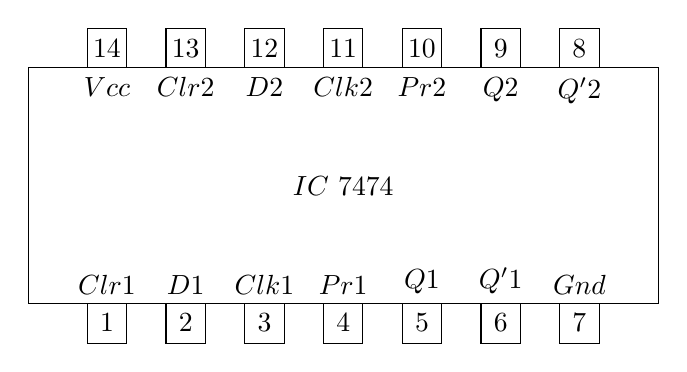
\begin{tikzpicture}                                           
	\draw (0,2) rectangle (8,5);                         
	\draw (4,3.5) node{$IC$ $7474$};                    
	\draw (0.75,2) rectangle (1.25,1.5);               
	\draw (1,2) node[below]{$1$};                        
	\draw (1,2) node[above]{$Clr1$};                     
	\draw (1.75,2) rectangle (2.25,1.5);                 
	\draw (2,2) node[below]{$2$};                      
	\draw (2,2) node[above]{$D1$};                        
	\draw (2.75,2) rectangle (3.25,1.5);                                                                        
	\draw (3,2) node[below]{$3$};                   
	\draw (3,2) node[above]{$Clk1$};                   
	\draw (3.75,2) rectangle (4.25,1.5);             
	\draw (4,2) node[below]{$4$};                 
	\draw (4,2) node[above]{$Pr1$};                      
	\draw (4.75,2) rectangle (5.25,1.5);                  
	\draw (5,2) node[below]{$5$};                        
	\draw (5,2) node[above]{$Q1$};                                                                               
	\draw (5.75,2) rectangle (6.25,1.5);                 
	\draw (6,2) node[below]{$6$};                        
	\draw (6,2) node[above]{$Q'1$};                      
	\draw (6.75,2) rectangle (7.25,1.5);               
	\draw (7,2) node[below]{$7$};                     
	\draw (7,2) node[above]{$Gnd$};                    
	\draw (0.75,5) rectangle (1.25,5.5);               
	\draw (1,5) node[above]{$14$};                      
	\draw (1,5) node[below]{$Vcc$};                    
	\draw (1.75,5) rectangle (2.25,5.5);                 
	\draw (2,5) node[above]{$13$};                       
	\draw (2,5) node[below]{$Clr2$};
                
		\draw (2.75,5) rectangle (3.25,5.5);               
		\draw (3,5) node[above]{$12$};                      
		\draw (3,5) node[below]{$D2$};                     
		\draw (3.75,5) rectangle (4.25,5.5);                
		\draw (4,5) node[above]{$11$};                       
		\draw (4,5) node[below]{$Clk2$};                    
		\draw (4.75,5) rectangle (5.25,5.5);               
		\draw (5,5) node[above]{$10$};
		\draw (5,5) node[below]{$Pr2$};                    
		\draw (5.75,5) rectangle (6.25,5.5);              
		\draw (6,5) node[above]{$9$};                       
		\draw (6,5) node[below]{$Q2$};                     
		\draw (6.75,5) rectangle (7.25,5.5);               
		\draw (7,5) node[above]{$8$};                      
		\draw (7,5) node[below]{$Q'2$};             
\end{tikzpicture}                                  

		\caption{7474}
		\label{fig:2}
	\end{figure}


The connections between the arduino and IC 7474 is as follows:
	\begin{table}[h]
		\begin{center}
			\begin{tabular}{|c|c|c|c|c|c|c|c|c|c|c|c|}
\hline  & \multicolumn{2}{|c|}{INPUT} & \multicolumn{2}{|c|}{OUTPUT} & \multicolumn{2}{|c|}{CLOCK} & \multicolumn{4}{|c|}{VCC} \\
\hline ARDUINO & D2 & D3 & D5 & D6 & \multicolumn{2}{|c|}{D13} & \multicolumn{4}{|c|}{5V} \\
\hline 7474 & 5 & 9 & 2 & 12 & 3 & 11 & 1 & 4 & 10 & 13 \\
\hline 7447 &  &  & 1 & 7 &  &  &  & 16 &  & \\
\hline
\end{tabular}

			\caption{connections}
			\label{table:3}
		\end{center}
	\end{table}


\section{Software}

The code to implement the above circuit is : \\

		\lstinputlisting{main.c}

\end{document}
